\documentclass[10pt,aspectratio=169]{beamer}

\usepackage[T1]{fontenc}
\usepackage{lmodern}
\usepackage{tikz}
\usetikzlibrary{arrows.meta,positioning,calc}

\definecolor{accent}{RGB}{76,73,210}
\definecolor{softblue}{RGB}{239,242,255}
\definecolor{darkgray}{RGB}{46,46,52}
\definecolor{midgray}{RGB}{102,102,112}

\setbeamercolor{normal text}{fg=darkgray,bg=white}
\setbeamercolor{structure}{fg=accent}
\setbeamercolor{frametitle}{fg=accent}
\setbeamercolor{block title}{fg=white,bg=accent}
\setbeamercolor{block body}{fg=darkgray,bg=softblue}
\setbeamerfont{frametitle}{size=\Large,series=\bfseries}
\setbeamertemplate{navigation symbols}{}
\setbeamertemplate{frametitle}{
  \vspace{0.2cm}
  \insertframetitle\par
  {\color{accent!35}\rule{\textwidth}{0.5pt}}
}
\setbeamertemplate{footline}{}

\begin{document}

% ============================================================
% 1. TITLE
% ============================================================

\begin{frame}[plain]
\vspace{1.3cm}
\begin{center}
{\fontsize{28}{32}\selectfont\color{accent}\bfseries K2 Escape\par}
\vspace{0.3cm}
{\large A Multi-Agent Survival Challenge\par}
\vspace{0.7cm}
{\color{accent!35}\rule{0.45\textwidth}{0.8pt}}
\vspace{0.6cm}

{\small Winnie Hsu \quad$\cdot$\quad Blythe \quad$\cdot$\quad Kate \quad$\cdot$\quad Wei Min\par}
\vspace{0.12cm}
{\small\color{midgray} University of Michigan \;$\cdot$\; K2 Horizon Hackathon}
\end{center}
\end{frame}

% ============================================================
% 2. GAME DESIGN
% ============================================================

\begin{frame}{Game Design: Can K2 Escape the Backrooms by Itself?}

{\color{midgray}\small No human player --- K2 Horizon controls the character from start to exit, in 180 seconds.}

\vspace{0.4cm}

\begin{center}
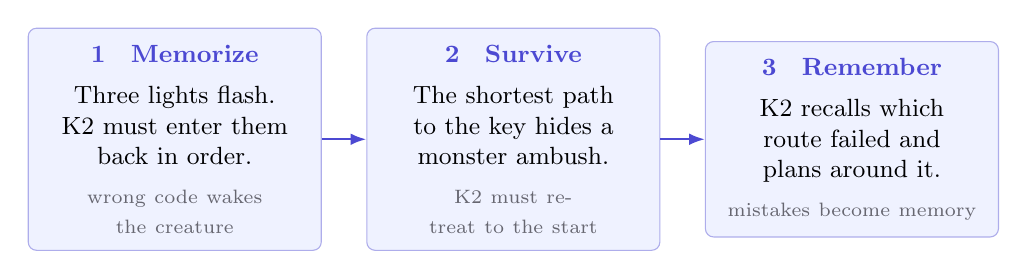
\begin{tikzpicture}[
  lvl/.style={draw=accent!45, fill=softblue, rounded corners=3pt,
    text width=3.3cm, minimum height=2.3cm, align=center, inner sep=6pt, font=\small},
  arrow/.style={-{Latex[length=2mm]}, thick, draw=accent}
]
\node[lvl] (l1) at (0,0) {\textbf{\color{accent}1 \; Memorize}\\[4pt]
  Three lights flash.\\ K2 must enter them\\ back in order.\\[3pt]
  {\scriptsize\color{midgray}wrong code wakes the creature}};
\node[lvl] (l2) at (4.3,0) {\textbf{\color{accent}2 \; Survive}\\[4pt]
  The shortest path\\ to the key hides a\\ monster ambush.\\[3pt]
  {\scriptsize\color{midgray}K2 must retreat to the start}};
\node[lvl] (l3) at (8.6,0) {\textbf{\color{accent}3 \; Remember}\\[4pt]
  K2 recalls which\\ route failed and\\ plans around it.\\[3pt]
  {\scriptsize\color{midgray}mistakes become memory}};
\draw[arrow] (l1) -- (l2);
\draw[arrow] (l2) -- (l3);
\end{tikzpicture}
\end{center}

\vspace{0.35cm}

\begin{block}{Core idea}
K2 decides \textbf{what to do}. The game engine decides \textbf{how to execute it}.
\end{block}

\end{frame}

% ============================================================
% 3. 3D FRONTEND
% ============================================================

\begin{frame}{Frontend: A Live 3D Backrooms}

\vspace{0.2cm}

\begin{columns}[t,onlytextwidth]
\column{0.47\textwidth}
{\color{accent}\bfseries First-person 3D world}
\begin{itemize}
  \setlength{\itemsep}{0.2cm}
  \item Flashlight POV in Backrooms halls
  \item A red-eyed creature on the chase
  \item \textbf{CORRECT / FAIL} pop-ups
\end{itemize}

\column{0.47\textwidth}
{\color{accent}\bfseries Watch the agents think}
\begin{itemize}
  \setlength{\itemsep}{0.2cm}
  \item Agents light up when called
  \item Live reasoning trace
  \item Live map with blocked routes
\end{itemize}
\end{columns}

\vspace{0.7cm}

\begin{center}
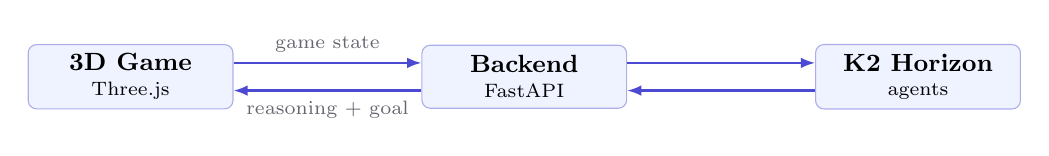
\begin{tikzpicture}[
  box/.style={draw=accent!45, fill=softblue, rounded corners=3pt,
    minimum width=2.6cm, minimum height=0.8cm, align=center, font=\small},
  arrow/.style={-{Latex[length=1.8mm]}, thick, draw=accent},
  lab/.style={font=\scriptsize, text=midgray}
]
\node[box] (g) at (0,0) {\textbf{3D Game}\\[-2pt]{\scriptsize Three.js}};
\node[box] (a) at (5,0) {\textbf{Backend}\\[-2pt]{\scriptsize FastAPI}};
\node[box] (k) at (10,0) {\textbf{K2 Horizon}\\[-2pt]{\scriptsize agents}};
\draw[arrow] ([yshift=5pt]g.east) -- node[lab,above]{game state} ([yshift=5pt]a.west);
\draw[arrow] ([yshift=-5pt]a.west) -- node[lab,below]{reasoning + goal} ([yshift=-5pt]g.east);
\draw[arrow] ([yshift=5pt]a.east) -- ([yshift=5pt]k.west);
\draw[arrow] ([yshift=-5pt]k.west) -- ([yshift=-5pt]a.east);
\end{tikzpicture}
\end{center}

\end{frame}

% ============================================================
% 3. MULTI-AGENT ARCHITECTURE
% ============================================================

\begin{frame}{Multi-Agent Architecture}

\begin{center}
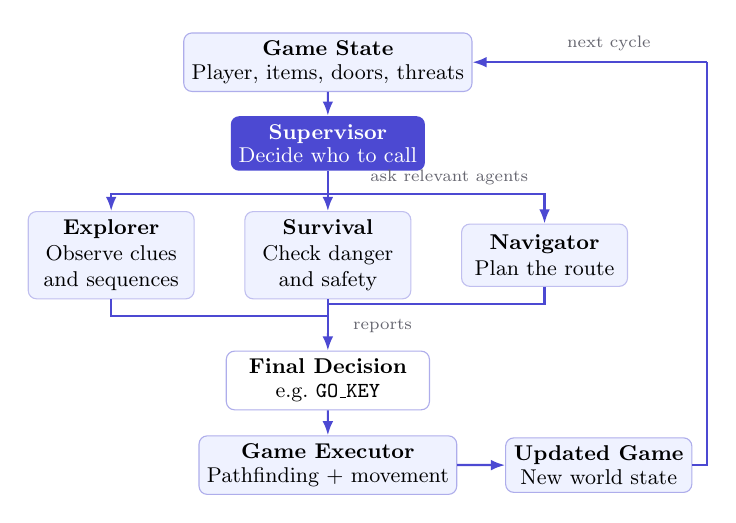
\begin{tikzpicture}[scale=0.86, transform shape,
  main/.style={draw=accent!45, fill=softblue, rounded corners=3pt,
    minimum width=2.75cm, minimum height=0.68cm, align=center, font=\small},
  supervisor/.style={draw=none, fill=accent, text=white, rounded corners=3pt,
    minimum width=2.75cm, minimum height=0.78cm, align=center, font=\small},
  specialist/.style={draw=accent!35, fill=softblue, rounded corners=3pt,
    minimum width=2.45cm, minimum height=0.92cm, align=center, font=\small},
  decision/.style={draw=accent!45, fill=white, rounded corners=3pt,
    minimum width=3.0cm, minimum height=0.78cm, align=center, font=\small},
  arrow/.style={-{Latex[length=1.8mm]}, thick, draw=accent},
  label/.style={font=\scriptsize, text=midgray}
]

\node[main] (game) at (0,0) {\textbf{Game State}\\[-1pt] Player, items, doors, threats};
\node[supervisor] (sup) at (0,-1.2) {\textbf{Supervisor}\\[-1pt] Decide who to call};
\draw[arrow] (game) -- (sup);

\node[specialist] (explorer) at (-3.2,-2.85) {\textbf{Explorer}\\ Observe clues\\ and sequences};
\node[specialist] (survival) at (0,-2.85) {\textbf{Survival}\\ Check danger\\ and safety};
\node[specialist] (navigator) at (3.2,-2.85) {\textbf{Navigator}\\ Plan the route};

\coordinate (branch) at (0,-1.95);
\draw[accent,thick] (sup.south) -- (branch);
\draw[arrow] (branch) -| (explorer.north);
\draw[arrow] (branch) -- (survival.north);
\draw[arrow] (branch) -| (navigator.north);
\node[label,anchor=south west] at (0.5,-1.93) {ask relevant agents};

\coordinate (merge) at (0,-4.0);
\draw[accent,thick] (explorer.south) -- ++(0,-0.25) -| (merge);
\draw[accent,thick] (survival.south) -- (merge);
\draw[accent,thick] (navigator.south) -- ++(0,-0.25) -| (merge);
\node[label,anchor=west] at (0.25,-3.9) {reports};

\node[decision] (decision) at (0,-4.7) {\textbf{Final Decision}\\[-1pt] e.g.\ \texttt{GO\_KEY}};
\draw[arrow] (merge) -- (decision);

\node[main] (executor) at (0,-5.95) {\textbf{Game Executor}\\[-1pt] Pathfinding + movement};
\draw[arrow] (decision) -- (executor);

\node[main] (updated) at (4.0,-5.95) {\textbf{Updated Game}\\[-1pt] New world state};
\draw[arrow] (executor) -- (updated);

\coordinate (loopright) at (5.6,-5.95);
\coordinate (looptop) at (5.6,0);
\draw[accent,thick] (updated.east) -- (loopright) -- (looptop);
\draw[arrow] (looptop) -- (game.east);
\node[label,anchor=south] at (4.15,0.05) {next cycle};
\end{tikzpicture}
\end{center}

\vspace{-0.1cm}
\begin{center}
{\small\color{accent}\bfseries Specialists advise. The Supervisor decides. The game acts.}
\end{center}

\end{frame}

\end{document}
